\documentclass{article}

\usepackage{graphicx}
\usepackage{amsmath}
\usepackage{fancyhdr}
\usepackage[sorting=none]{biblatex}
\usepackage[margin=1in]{geometry}
\usepackage[font={small,it}]{caption}
\usepackage{placeins}
\usepackage{xepersian}

%\DeclareMathOperator*{\btie}{\bowtie}
\addbibresource{bibliography.bib}
\settextfont[Scale=1.2]{B-NAZANIN.TTF}
\setlatintextfont[Scale=1]{Times New Roman}
\renewcommand{\baselinestretch}{1.5}
\pagestyle{fancy}
\fancyhf{}
\rhead{تکلیف دوم ورزش 1}
\lhead{\thepage}
\rfoot{علیرضا ابره فروش}
\lfoot{9816603}
\renewcommand{\headrulewidth}{1pt}
\renewcommand{\footrulewidth}{1pt}

\begin{document}
\begin{titlepage}
\begin{center}
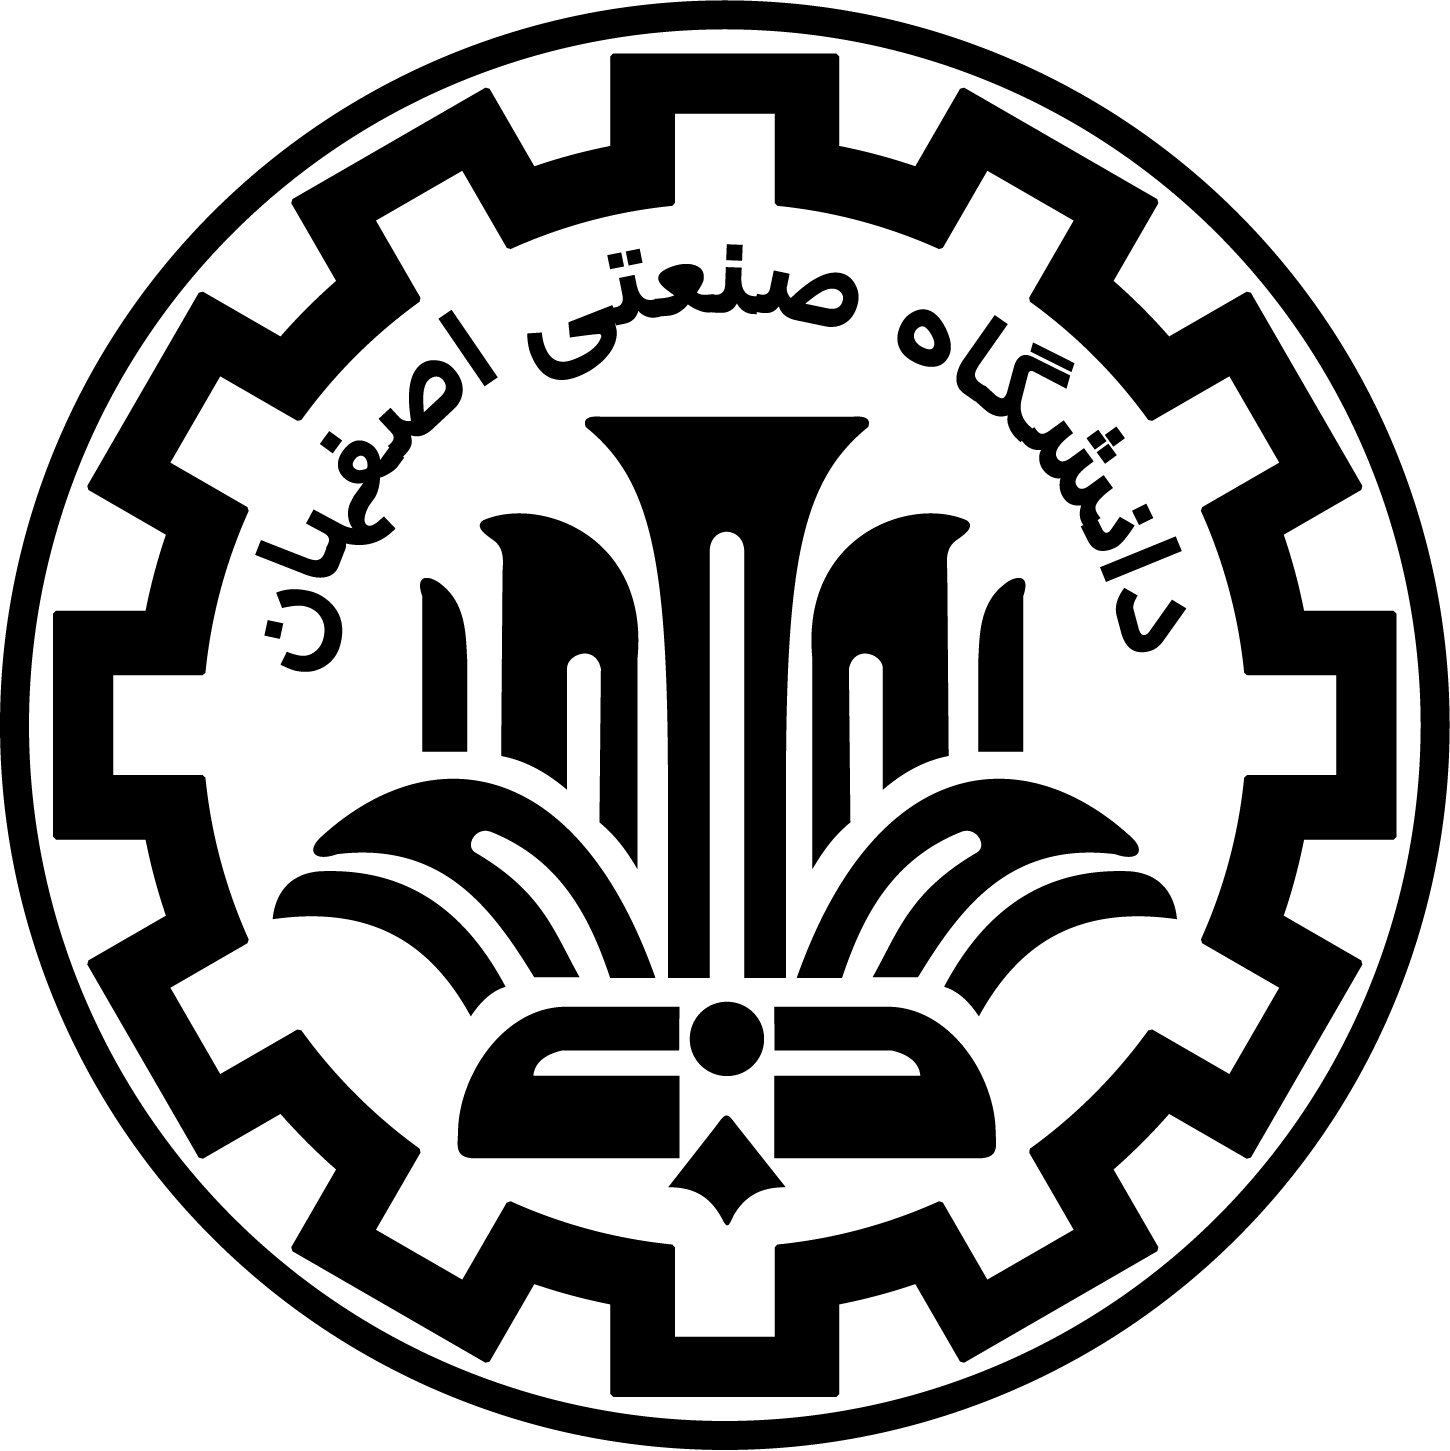
\includegraphics[width=0.4\textwidth]{figures/IUT Logo.png}\\
        
\LARGE
\textbf{دانشگاه صنعتی اصفهان}\\
\textbf{دانشکده مهندسی برق و کامپیوتر}\\
        
\vfill
        
\huge
\textbf{عنوان: تکلیف چهارم درس ریزپردازنده}\\
        
\vfill
        
\LARGE
\textbf{نام و نام خانوادگی: علیرضا ابره فروش}\\
\textbf{شماره دانشجویی: 9816603}\\
\textbf{نیم\,سال تحصیلی: پاییز 1400}\\
\textbf{مدرّس: دکتر عارف کریمی افشار}\\
\end{center}
\end{titlepage}


%\tableofcontents
\newpage
\begin{itemize}
    \item [$\bullet$]
اگر درحال کار با کامپیوتر هستیم سر به گونه‌ای باید مقابل مانیتور قرار بگیرد که زاویه دید ما بر مانیتور تقریبا عمود باشد.
	\item [$\bullet$]
هنگامی که دست‌ها بر روی میز قرار گرفته اند، زاویه آرنج حدودا باید 90 درجه باشد. درصورت اجبار تا 60 درجه هم مشکلی ندارد.
	\item [$\bullet$]
دست‌ها باید در راستای شانه قرار بگیرند و نباید به داخل یا خارج متمایل شوند. درصورتی که این اتفاق افتاد با انجام حرکت قرینه‌ی آن(یعنی خارج یا داخل) می‌توان اثرات ناشی از حرکت نادرست را جبران کرد.
	\item [$\bullet$]
اگر سر برای مطالعه به سمت پایین خم شود پس از 30 تا 45 دقیقه سر را به عقب هدایت کنید تا دچار درد گردن نشوید.
	\item [$\bullet$]
موقع نشستن روی صندلی به آن تکیه ندهید و مقداری به جلو خم شوید و دست‌هایتان را اهرم کنید.
	\item [$\bullet$]
هنگام نشستن راستای شانه‌ها با خطی که از بر وسط کتف عمود است باید تشکیل یک به‌علاوه(+) بدهند. درصورتی که مجبور به به‌هم ریختن این به‌علاوه شدید برای رفع اثرات ناشی از حرکت نادرست، قرینه‌ی آن را انجام دهید.
	\item [$\bullet$]
لگن و پاها باید همزمان با تنه بچرخند و زانوها و شانه‌ها باید در یک راستا قرار بگیرند.
	\item [$\bullet$]
زانو‌ها حین انجام کار می‌توانند در ارتفاعی برابر یا کمی بالاتر از لگن قرار بگیرند.
	\item [$\bullet$]
می‌توان یک جاپایی در زیر میز قرار داد تا پنجه‌ها کمی به سمت ساق متمایل شود.

\end{itemize}



\end{document}
